\documentclass[11pt]{article}
\usepackage{graphicx}
\usepackage{fixltx2e}
\graphicspath{ {images/} }


\title{Literary Review}
\author{Michiel Willems}


\begin{document}
	

	
\maketitle

\section{OBD Overview}

\subsection{OBD purpose}

The goal of OBD2 is to Help Technicians Properly Diagnose and Repair Complex Problems \cite{OBDOverview}. To do this the protocol introduces:
\begin{itemize}
	\item Standardisation: information is communicated in s standardized format to allow for 1 tool to be used on many vehicles.
	\item Certification: Every vehicle manufacturer required to submit certification application for review and approval, which includes a detailed description of how the OBD2 protocol was implemented.
	\item Helps lowering emissions by identifying emission controls in need of repair.
\end{itemize}

\subsection{Fault Detection}
Every vehicle has a couple of specific values that don't change, and act as a kind of signature for each specific vehicle.
These include\cite{OBDOverview}:
\begin{itemize}
	\item The vehicle identification number (VIN).
	\item Readiness profile: A given make/model/year should have a specific readiness profile.
	\item ECU address allocation should be unique.
\end{itemize}
If a change in value of this data is detected, this could indicate possible fraud. Other so called 'fingerprinting' techniques are the CAL ID and CVN (which are also make/model/year specific), the communications protocol used (e.g. LIN, CAN, MOST and FLexRay) and the parameter ID's which are supported inside the vehicle. 

\section{Security, Vulnerability and Protection of Vehicular On-board Diagnostics}

\subsection{Threats}

Automobile hacking has become one of the major concerns for software security today. The attacker can take control of your car and its various features and functions without having physical access to the car. Everyday a new method of hacking is developed, which challenges the existing security solutions \cite{Yadav16}. Currently four out of ten car thefts in major cities involve some form of car hacking. Immobilisers used in 100 different models from the likes of Volvo, VW, Audi and Fiat – especially models that come with a starter button instead of a key – were found vulnerable to hacking by thieves with access to a computer. The researchers were banned from publishing the report for two years by car manufacturers due to its sensitive nature. \cite{Saarinen}.

\subsection{Points of Entry}

\subsubsection{Physical}

\begin{itemize}
	\item Ripping apart the dashboard.
	\item \textbf{Door Locks and Key Fobs:} Since 1995 EU legislation demands that all new cars come standard with an electronic immobiliser. This device only allows the vehicle to start when it is provided the right credentials - but thieves can wirelessly steal all of the information from a car key in seconds. \cite{Yadav16}
\end{itemize}

\subsubsection{Wireless}

\begin{itemize}
	\item \textbf{Bluetooth:}
	\item \textbf{Cd Player:}
	\item \textbf{Tire Pressure Monitoring System:}
	\item \textbf{Unauthorized applications:}
\end{itemize}

\subsection{OBDII port}

In order to provide comprehensive, easy-to-use self diagnostic and reporting functionality for in vehicle ECUs, a standardized On-Board Diagnostic (OBD) interface was developed in the 1990s and today OBD is deployed worldwide and legally mandatory in the US and Europe. \cite{Yadav16} On one hand, OBD enables digital access to public data, for instance to emission control and error codes and on the other hand, OBD enables access also to “hidden” manufacturer-specific ECU settings, for instance to theft protection or engine control \cite{Yadav16}.

\subsection{OBD port threats}
It has been found out that a set of messages and signals that could be sent on car‟s CAN bus (via OBD-II) to control key components (e.g. lights, locks, brakes, and engine) as well as injecting code into key ECUs to insert persistent capabilities and to bridge across multiple CAN buses [13]. Due to commonly available tools and information, automotive manufacturers face an increasing amount of ECU manipulations that might affect vehicle safety, legal applications (e.g., exhaust gas treatment) or undermine aftermarket business models. Furthermore, critical data are stored in the ECUs such as crash data, data for insurances, or warranty indicators. Such data is also very attractive for malicious manipulations. For example, data such as vehicle speed, seat belt status, brake pedal position etc. are typically recorded in the seconds before a crash. A driver who has been involved in an accident could be motivated to change the recorded data to indicate that the brakes were applied when they really were not.


\subsection{Security Solutions}

\subsubsection{Seed Key Algorithm}

The seed key algorithm (like the name implies) applies a secret key value to calculate the response key from the seed. Only the person with the correct secret key can gain access to the diagnostic service of a specific ECU. The problem with this algorithm is the fact the same ECU in different cars will have the same secret key. Another problem is that the secret key material is often stored in unprotected memory. If enough keys are made public this would undermine the security of the entire algorithm.  

\subsubsection{Two-Way authentication method}

This algorithm is an extension of the seed-key algorithm. In addition to requiring possession of the secret key, a message will be sent to the client of the vehicle whenever access is requested (Cellular or via Internet). Without acknowledgement from the user the seed is dropped and access is denied. The above process adds a layer of safety as a result of keeping the client informed at every stage.

\subsubsection{Timer Method} 

The timer method is again an extension of the Two-Way authentication method. It Exploits the time brute force methods and other algorithms take to crack a 16-bit long seed key, as well as giving more autonomy the car owner by giving the global seed directly to the client, who in turn must enter the key to complete the authentication process. As soon as a security access request is sent by the tester, the timer will be started. As soon as the timer runs out, a message or a notification alert is sent to the client informing about the malicious activity, as well as aborting the authentication process.

\section{Security Crash Test – Practical Security Evaluations of Automotive Onboard IT Components}

\subsection{Threats}

\begin{itemize}
	\item manipulating the steering wheel or brakes.
	\item distracting the driver by triggering odd vehicle behaviour.
	\item odometer manipulation.
	\item changing crash data, data for insurances, or warranty indicators.
	\item access to private data such as vehicle location, credentials to online services, or mobile payment data
	\item theft of vehicles or valuable vehicle components such as airbags or head units, e.g. by abusing diagnostics commands to reprogram a new key.
\end{itemize}

\subsection{Automotive Security Assurance Levels}

In 2015 Stephanie Bayer, Thomas Enderle, Dennis Kengo Oka and Marko Wolf introduced the "Automotive security evaluation assurance levels” (ASEAL) which define up to four discrete security testing levels that determine (i) the size of security evaluation scope, that means which security analyses and tests have to be executed for a certain ASEAL and (ii) how “deeply” and thoroughly these security analyses and tests have to be executed. The goal for ASEAL is to make security evaluations comparable and, in consequence, to make it possible to assign standardized levels of minimum security assurance to each automotive onboard IT component. \cite{Bayer15} A comprehensive summary of the proposed levels is shown in figure \ref{fig:aseal}.

\begin{figure}[h]
	\caption{ASEAL levels.}
	\label{fig:aseal}
	\centering
	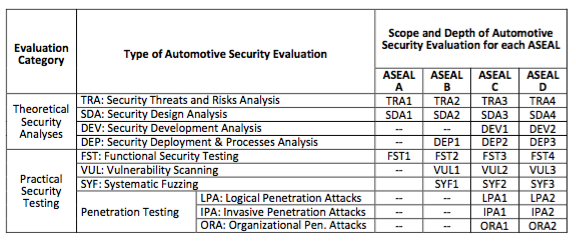
\includegraphics[width=\textwidth]{ASEAL.png}
\end{figure}




\section{On Board Diagnostics: Risks and Vulnerabilities of the Connected Vehicle}

The OBD-II port was created to provide consumers with choice and control over their purchase. At the same time, this freedom must be balanced with thoughtful conversations on how to limit adversaries’ access to vehicle internals

\subsection{Recommendations for security of IT components in cars.}

\begin{itemize}
	\item \textbf{Separate CAN communication from the network stack:} The OBDII data that is sent should separated from the network stack and allow an application to send a request only from a list of pre- chosen OBD-II commands.
	
	\item \textbf{Sign and encrypt firmware updates:} Firmware updates should always be cryptographically signed and encrypted to prevent firmware modification by an attacker.
	
	\item \textbf{Be secure by default:} It is recommended that every third-party device that ends up in the vehicle (e.g. ECU's developed in another factory) is shipped in the most secure configuration. The reseller can then modify the configuration as needed.
	
	\item \textbf{Obey the principle of least privilege:} Additional features introduce additional risk. This means that every device should only implement just enough connectivity to perform it's desired function. 
\end{itemize}



\subsection{The connected car infrastructure}

The connected car can be described as a vehicle with one or more external wireless commu- nication possibilities, which connects the vehicle to an external network. These external networks can have many different configurations (e.g. local network vs connection to the internet) and purposes (e.g. remote diagnostics, software download, media streaming, etc). Figure \ref{fig:concar} shows the infrastructure of the common connected car. vehicular communication can be divided into 2 groups:  Vehicle-to-vehicle (V2V) and Vehicle-to-Infrastructure (V2I) communication, collectively known as Vehicle-to-X
(V2X) communication. The network can also be implemented in a couple of ways: Wifi-technology, Cellular communications and others (e.g. WAVE- or ETSI ITS-protocol).

\begin{figure}[h]
	\caption{Connected car infrastructure}
	\label{fig:concar}
	\centering
	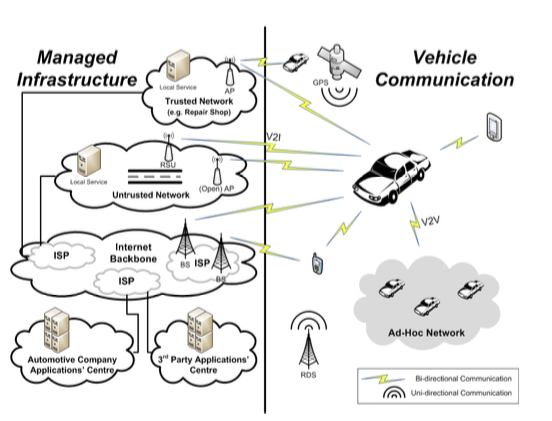
\includegraphics[width=\textwidth]{ConnectedCar}
\end{figure}

\subsection{ISO 13400 — Diagnostics over IP (DoIP)}

DoIP uses IP, TCP, and UDP, both in unicast and broadcast. The diagnostics messages themselves are not specified by DoIP as it's purpose is to transmit these messages over IP-based networks. Figure \ref{fig:doip} shows the protocol stack of the DoIP protocol. \cite{ISO13400}

\begin{figure}[h]
	\caption{DoIP protocol stack}
	\label{fig:doip}
	\centering
	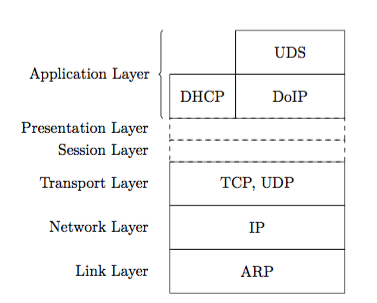
\includegraphics[width=\textwidth]{DOIP}
\end{figure}

\subsection{ISO 14229 — Unified Diagnostic Services (UDS)}

ISO 14229 defines an application layer protocol for diagnostics of vehicles. 26 services are provided and with these services, it is possible to read and write data to ECUs, reset ECUs, and upload firmware. \cite{ISO14229}

\section{An In-Depth Analysis of the Security of the Connected Repair Shop}

In 2015 Pierre Kleberger, Tomas Olovsson, and Erland Jonsson of the Department of Computer Science and Engineering of Chalmers University of Technology
in Gothenburg, Sweden, presented a security analysis of connected repair shops. They used the model given in figure \ref{fig:repshop}. After a detailed analysis of possible threats (using the threat, vulnerability, and risk analysis (TVRA) method defined by ETSI.) they came up with the following security countermeasures \cite{Kleberger15}.

\begin{itemize}
	\item Data should be stored and transmitted encrypted.
	\item Strong authentication is needed. Private/public keys, with or without certificates, and Kerberos-like authentication mechanisms can be used.
	\item Traffic separation should occur in the repair shop network. This helps in dealing with misbehaving software and helps contain software bugs. Traffic seperation can be logical (e.g. VLAN technology) or cryptographical (e.g. using cryptographic keys and encryption to separate traffic). Cryptographic encryption is preferred since it is more flexible.
	\item Digital signatures and message authentication codes (MACs) can be used to verify the source of and the integrity in the communication.
	\item Timestamps  can be used to prevent replay attacks.
\end{itemize}

All of these countermeasures are clearly applicable to other V2I and V2X models (e.g. automatic gas payment, V2V data sharing, etc).

\begin{figure}[h]
	\caption{Connected Repair Shop Infrastructure}
	\label{fig:repshop}
	\centering
	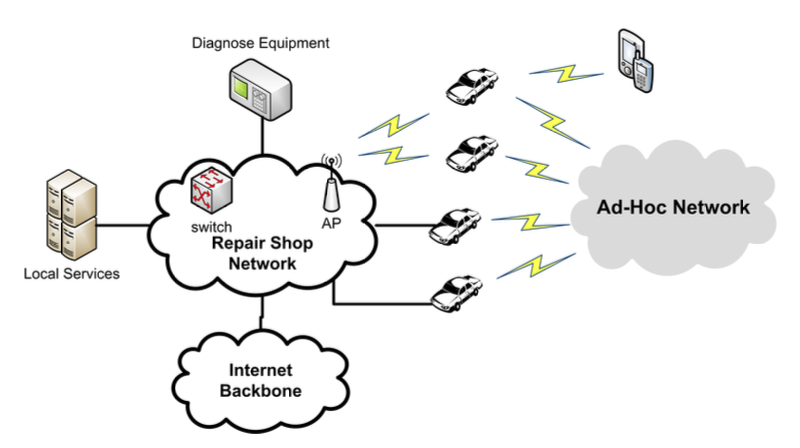
\includegraphics[width=\textwidth]{repairshop}
\end{figure}

\section{Comprehensive Experimental Analyses of Automotive Attack Surfaces}

\subsection{access}

\begin{itemize}
	\item Entertainment: Disc, USB and iPod.
	\item Remote Keyless Entry.
	\item RFID car keys.
	\item Emerging short-range channels: A number of manufacturers have started incorporating 802.11 WiFi in their automobiles.
	\item Dedicated Short-Range Communications (DSRC) standard: In such systems, forward vehicles communicate digitally to trailing cars to inform them of sudden changes in acceleration to support improved collision avoidance and harm reduction.
	\item broadcast channels: The modern automobile includes a plethora of broad- cast receivers for long-range signals: Global Positioning System (GPS), Satellite Radio, Digital Radio, and the Radio Data System (RDS) and Traffic Message Channel (TMC) signals transmitted as digital subcarriers on existing FM-bands.
	\item Addressable Channels: Perhaps the most important part of the long-range wireless attack surface is that exposed by the remote telematics systems (e.g. cellular).
\end{itemize}

\begin{figure}[h]
	\caption{Attack surface capabilities}
	\label{fig:atksrfc}
	\centering
	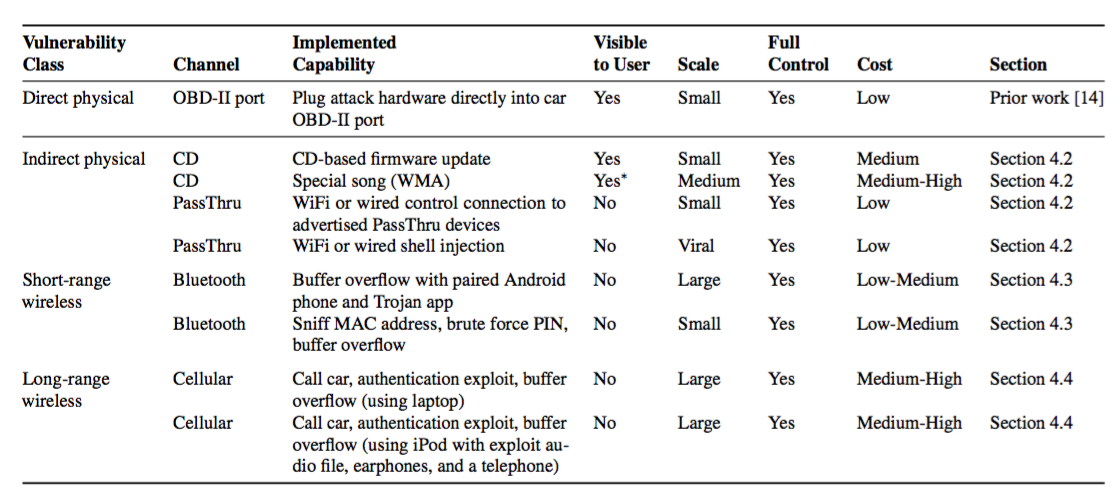
\includegraphics[width=\textwidth]{AttackSurface}
\end{figure}

Figure \ref{fig:atksrfc} shows a summary of the attack surface capabilities of each of the entry points discussed earlier.

\section{CANtoolz}

\cite{Sintsov}

\section{Securing the Automobile: a Comprehensive Approach}

In particular, the CAN bus, one of the primary buses used in modern automobiles, is not particularly safe or se- cure. There is no protection against “babbling idiots” on the bus, in which a node denies service to other nodes, either because of a fault or in a malicious denial of service.

\section{On securing the connected car}

\subsection{Automotive business constraints}

Business constraints can be in tension with developing secure systems, particularly those that have a great impact on cost, in \cite{Pike15} a couple of constraints are highlighted:

\begin{itemize}
	\item Part cost.
	\item Size and weight (especially when available space is limited, e.g. sports cars).
	\item Legacy integration: Since car components are designed to have long lifetimes, a lot of new designs might have to communicate with legacy components.
	\item Timing requirements: Additional security measures might violate timing constraints.
	\item Standardisation: A single manufacturer cannot always afford to break away from industry standards in order to improve security.
\end{itemize}

They also propose a couple of changes to the ECU supplier model in order to make automobiles more secure:

\begin{itemize}
	\item Independent evidence: Car Manufacturers should require independent evidence that security objectives are met by a supplier’s software. 
	\item Collaboration: The security of the manufactured car will improve if the third party suppliers are allowed to embed their own engineers within the manufacturing team.
	\item Open software: This might seem counter-intuitive but open software is subject to public analysis, which in turn should reveal any vulnerabilities, thereby improving it's security.
	\item Liability: Finally, there is precedent for holding automotive manufacturers liable for harm caused by their software \cite{Precedent}.
\end{itemize}

They also propose some ways of improving the software of ECU's:

\begin{itemize}
	\item Software Development: A couple of improvements in the development of software are proposed: \begin{itemize}
		\item Coding Standards (e.g. MISRA C standard \cite{MISRA}).
		\item Static Analysis (static analyzers traverse the source code of a program and alert the user to possible flaws).
		\item Memory Safe Programming (e.g. use safe programming languages like RUST).
	\end{itemize}
	\item Testing:
	\begin{itemize}
		\item Fuzz testing (random testing input).
		\item property based testing (testing data generated in accordance with property specification, e.g. QuickCheck \cite{Quickheck}).
	\end{itemize}
	\item Formal Verification: \begin{itemize}
		\item Program Verifiers (e.g. Verifast \cite{Verifast}).
		\item Glue code generation.
	\end{itemize}
	\item Runtime Assurance: \begin{itemize}
		\item System Specialization (least privilege).
		\item Data Integrity.
		\item Runtime Verification (formal verification + testing).
		\item Software Fault Containment Regions.
	\end{itemize}
	\item Sanitizing inputs: \begin{itemize}
		\item Radio systems.
		\item Media systems.
		\item Telematics systems.
		\item Wireless key systems.
		\item Vehicle to Vehicle Communication.
	\end{itemize}
\end{itemize}

\section{Scalable CAN security for CAN, CANopen and other protocols}

\subsection{CANcrypt}

CANcrypt uses a CAN feature that allows two devices to exchange a hidden bit that is not visible to other CAN devices. This allows generating pairing keys that only the two devices know. CANcrypt uses a dynamic 64-bit key to cover the longest possible secure data block, 8 bytes. From this key, a pseudo one-time pad is generated and changes frequently. CANcrypt does not protect against DOS attacks.\cite{Pfeiffer}

\section{VulCAN: E icient Component Authentication and So ware Isolation for Automotive Control Networks}

In December of 2017 three researchers (Jo Van Bulck, Jan Tobias Mühlberg and Frank Piessens) at the KULeuven university in belgium, presented VulCAN. VulCAN is a generic design for vehicular message authentication, software component attestation and isolation. Their solution is distinguished from previous work (e.g. CANcrypt\cite{Pfeiffer}, VetiCAN\cite{VatiCAN} and Leia\cite{Leia}) by relying on trusted hardware and a minimal Trusted Computing Base (TCB). This TCB relies heavily on the SANCUS\cite{Sancus} security architecture (also developed at KuLeuven).

\subsection{SANCUS}

Many embedded platforms lack the standard security features (e.g. privilege levels and  virtual memory) present in high-end processors. SANCUS was developed to tackle this problem. the goal of SANCUS is to provide network embedded systems with remote attestation and strong integrity and authenticity guarantees with a minimal hardware TCB. Figure \ref{fig:sancus} shows the SANCUS system model. The infrastructure provider (IP) provides a number of nodes (N\textsubscript{i}) on which software providers (SP\textsubscript{i}) can deploy software modules SM\textsubscript{j,k}. This model is applicable to many ICT systems today (in the case of VulCAN this system of course a CAN network). Any system that supports installation of software modules by several software providers must implement measures to make sure that the different modules can not interfere with each other in undesired ways. To enforce this requirement SANCUS provides 4 security properties:

\begin{figure}[h]
	\caption{SANCUS system model}
	\label{fig:sancus}
	\centering
	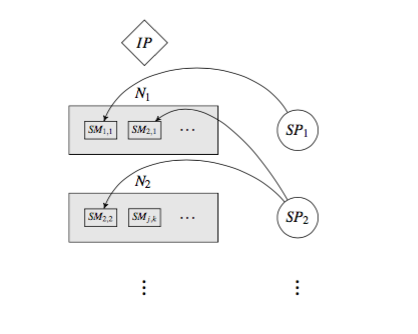
\includegraphics[width=\textwidth]{SANCUS}
\end{figure}

\begin{itemize}
	\item \textbf{Software module isolation:} Every software module has a runtime state that is not modifiable by other modules. The only way other modules are able to interact with it is by calling one of its designated entry points.
	\item \textbf{Remote attestation:} A software provider can verify with sufficient assurance that a specific software module is loaded on a specific node.
	\item \textbf{Secure communication:} A software provider can communicate with a software module while authenticity, integrity and freshness guarantees are maintained.
	\item \textbf{Secure linking:} A software module on a node can link to and call another module on the same node without interference by other software on the same node.
\end{itemize}

For more information on SANCUS confer \cite{Sancus}.

\subsection{VulCAN}

VulCAN was designed to compartmentalise every ECU into a small group of trustworthy authenticated software components (It's easy to see that this is where the SANCUS design was implemented). Figure \ref{fig:vulcan} shows An example CAN network scenario where an authenticated trusted path is set up between a software component that senses a braking pedal and wheel rotations, over an Anti-lock Braking System (ABS) component, all the way to a brake hydraulic actuator component. To fulfil the requirements of such a system VulCAN complies to the following requirements:

\begin{figure}[h]
	\caption{VulCAN example \cite{VulCAN}}
	\label{fig:vulcan}
	\centering
	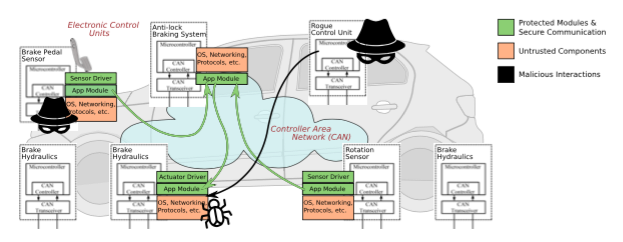
\includegraphics[width=\textwidth]{VulCAN}
\end{figure}

\begin{itemize}
	\item \textbf{Message Authentication:} The system uses MAC's (message authentication codes) to prove the message was indeed sent by a trusted sender component.
	
	\item \textbf{Lightweight Cryptography:} Lightweight cryptography is a must because of strict timing constraints (e.g. it is obvious that the example used in figure \ref{fig:vulcan} should perform as fast as possible) and because of the computational limitations of the embedded devices.
	
	\item \textbf{Replay Attack Resistance:} the authentication scheme is immune to replay attacks (a malicious agent injecting a previously sent message in the hope of it being falsely authenticated). This is ensured by using short term session keys, and a monotonically increasing counter or nonce as a source of freshness in the MAC computation.
	
	\item \textbf{Backwards Compatibility:} Legacy unmodified applications without authenticated communication should continue to function. To this end the system broadcasts the authenticated message in plain text, and afterwards constructs and transmits authentication data on a different CAN identifier, effectively decoupling the authentication metadata from the original message. 	
\end{itemize}

While the above requirements are mostly met by two other recent CAN authentication protocols \cite{Leia} \cite{VatiCAN}, a number of system-level guarantees were added for the system to be applicable in an in-vehicle CAN network:

\begin{itemize}
	\item \textbf{Real Time Compliance:} the system adheres to stringent real-time deadlines.
	\item \textbf{Component Isolation:} Effectively what SANCUS guarantees.
	\item \textbf{Component Attestation:} Also Guaranteed by SANCUS.
	\item \textbf{Dynamic Key Update:} It is possible for broken ECUs to be replaced at a distrusted automobile repair shop (again this is where SANCUS comes in).
\end{itemize}

To learn more about VulCAN confer \cite{VulCAN}.

\section{Security and privacy in vehicular communications: Challenges and opportunities
}

\subsection{Safety Requirements}
The ISO 26262 \cite{ISO-26262-1} standard defines the functional safety requirements that must apply during the complete lifecycle of every automotive electronic/electrical system that is safety-related. Among others (cf \cite{ISO-26262-1}) it introduces the Safety Integrity Level (ASIL), a risk-based approach to determine potential hazard in a vehicle operating scenario. There are four levels: ASIL-A, ASIL-B, ASIL-C and ASIL-D. The risk increases from ASIL-A to ASIL-D, where the ASIL-A level indicates the lowest risk while the ASIL-D level is the highest one.\cite{crispo}

\subsection{AUTOSAR}
AUTOSAR is a software architecture for the automotive sector. This architecture aims to assist with the development of vehicular software. 

\subsection{Different Communication protocols used inside vehicles}

\begin{figure}[h]
	\caption{Different data communication buses in modern cars \cite{crispo}}
	\label{fig:buses}
	\centering
	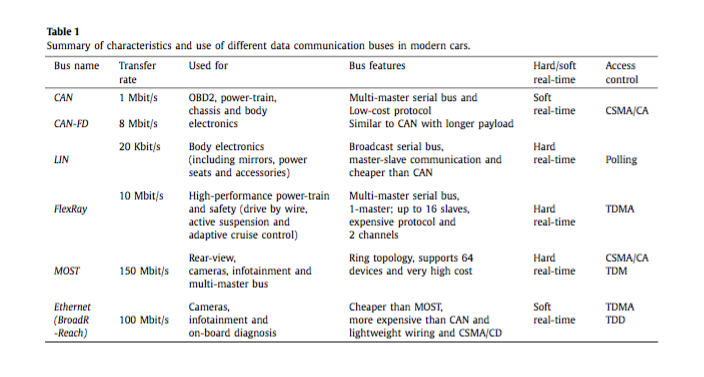
\includegraphics[width=\textwidth]{buses}
\end{figure}








\begin{thebibliography}{10}
	
	\bibitem{Pike15}
	Lee Pike, Jamey Sharp, Mark Tullsen, Patrick C. Hickey and James Bielman, \textit{Securing the automobile: A comprehensive approach}, 2015.
	
	\bibitem{Klinedinst05}
	Dan Klinedinst, Christopher King, 
	\textit{On Board Diagnostics: Risks and Vulnerabilities of the Connected Vehicle}, 2016.
	
	\bibitem{Kleberger15}
	Pierre Kleberger, \textit{On Securing the Connected Car},
	2015.
	
	\bibitem{Russel17}
	Brian Russell, Aaron Guzman, Paul Lanois, Drew Van Duren,
	\textit{Observations and Recommendations on Connected Vehicle Security},
	Cloud Security Alliance Internet of Things Working group, 2017.
	
	\bibitem{MillerA}
	Charlie Miller, Chris Valasek,
	\textit{A Survey of Remote Automotive Attack Surfaces}, 2015.
	
	\bibitem{Yadav16}
	Aastha Yadav, Gaurav Bose, Radhika Bhange, Karan Kapoor, N.Ch.S.N Iyengar, Ronnie D. Caytiles, \textit{Security, Vulnerability and Protection of Vehicular On-board Diagnostics}, 2016.
	
	\bibitem{ODBwiki}
	https://en.wikipedia.org/wiki/On-board\textunderscore diagnostics.
	
	\bibitem{PIDwiki}
	https://en.wikipedia.org/wiki/OBD-II\textunderscore PIDs.
	
	\bibitem{CANwiki}
	https://en.wikipedia.org/wiki/CAN\textunderscore bus.
	
	\bibitem{MillerB}
	Charlie Miller, Chris Valasek,
	\textit{CAN Message Injection},
	OG Dynamite Edition
	, 2016.
	
	\bibitem{MillerC}
	Charlie Miller, Chris Valasek,
	/textit{Adventures in Automotive Networks and Control Units}.
	
	\bibitem{Washington}
	Stephen Checkoway, Damon McCoy, Brian Kantor, Danny Anderson, Hovav Shacham, and Stefan Savage University of California, San Diego
	Karl Koscher, Alexei Czeskis, Franziska Roesner, and Tadayoshi Kohno,
	University of Washington
	\textit{Comprehensive Experimental Analyses of Automotive Attack Surfaces}.
	
	\bibitem{Bayer15}
	Stephanie Bayer, Thomas Enderle, Dennis Kengo Oka , Marko Wolf.
	\textit{Security Crash Test – Practical Security Evaluations of Automotive Onboard IT Components}, 2015.
	
	\bibitem{Enisa}
	European Union Agency for Network and Information Security (ENISA),
	\textit{Cyber Security and Resilience of smart cars},
	2016.
	
	\bibitem{OBDOverview}
	Allen Lyons, California Air Resources Board ,
	\textit{On-Board Diagnostics (OBD) Program Overview},
	2015 .
	
	\bibitem{Saarinen}
	Marien Saarinen, http://www.autoexpress.co.uk/car-news/consumer-news/92304/car-hacking-study-shows-over-100-models-at-risk, 
	\textit{Car hacking: study shows over 100 models at risk},
	2015.
	
	\bibitem{ISO14229}
	\textit{ISO 14229-1:2013: Road vehicles — Unified diagnostic services (UDS) — Part 1: Specification and requirements.}
	ISO, 2013.
	
	\bibitem{ISO13400}
	\textit{ISO 13400-1:2011: Road vehicles — Diagnostic communication over Internet Protocol (DoIP) — Part 1: General information and use case definition.} ISO, 2011.
	
	\bibitem{Sintsov}
	Alexei Sintsov, 
	\textit{(pen)testing vehicles with CANToolz},
	2016.
	
	\bibitem{Precedent}
	Philip Koopman. \textit{A case study of toyota unintended acceleration and software safety.} Public seminar, September 2014.
	
	\bibitem{MISRA}
	\textit{Guidelines for the Use of the C Language in Critical Systems.} MISRA, 2004.
	
	\bibitem{Quickheck}
	Koen Claessen and John Hughes. 
	\textit{QuickCheck: A lightweight tool for random testing of haskell programs.} In Proceedings of the Fifth ACM SIGPLAN International Conference on Functional Programming, ICFP ’00, pages 268–279. ACM, 2000.
	
	\bibitem{Verifast}
	Bart Jacobs, Frank Piessens,
	\textit{The VeriFast Program Verifier}, Department of Computer Science, Katholieke Universiteit Leuven, Belgium.
	
	\bibitem{Pfeiffer}
	Olaf Pfeiffer, Christian Keydel, 
	\textit{Scalable CAN security for CAN, CANopen and other protocols}, 2017.
	
	\bibitem{Sancus}
	Job Noorman, Pieter Agten ,Wilfried Daniels ,Raoul Strackx
	Anthony Van Herrewege, Christophe Huygens, Bart Preneel, Frank Piessens
    ,Ingrid Verbauwhede, \textit{Sancus: Low-cost trustworthy extensible networked devices with a zero-software Trusted Computing Base}, iMinds-DistriNet and iMinds-COSIC, KU Leuven.
    
    \bibitem{VulCAN}
    Jan Tobias Mühlberg, Frank Piessens, Jo Van Bulck,
    \textit{VulCAN: E icient Component Authentication and So ware Isolation for Automotive Control Networks}, Imec-Distrinet KuLeuven, 2017.
    
    \bibitem{Leia}
    Andreea-Ina Radu, Flavio D. Garcia,
    \textit{LeiA: A Lightweight Authentication Protocol forCAN},
    School of Computer Science,University of Birmingham, UK.
    
    \bibitem{VatiCAN}
    Stefan N ̈urnberger, Christian Rossow,
    \textit{vatiCAN, Vetted, Authenticated CAN Bus},
	CISPA, Saarland University, Germany.
	
	\bibitem{ISO-26262-1}
	ISO-26262-1, Road vehicles — Functional Safety, ISO 26262-1, International Or- ganization for Standardization, Geneva, Switzerland, 2011.
	
	\bibitem{crispo}
	Cesar Bernardini, Muhammad Rizwan Asghar, Bruno Crispo,
	\textit{Security and privacy in vehicular communications: Challenges and opportunities}, 2017.

	
\end{thebibliography}

\end{document}

